% !TEX TS-program = XeLaTeX
% use the following command:
% all document files must be coded in UTF-8
\documentclass[portuguese]{textolivre}
% build HTML with: make4ht -e build.lua -c textolivre.cfg -x -u article "fn-in,svg,pic-align"

\journalname{Texto Livre}
\thevolume{16}
%\thenumber{1} % old template
\theyear{2023}
\receiveddate{\DTMdisplaydate{2023}{8}{1}{-1}} % YYYY MM DD
\accepteddate{\DTMdisplaydate{2023}{10}{21}{-1}}
\publisheddate{\DTMdisplaydate{2023}{11}{20}{-1}}
\corrauthor{Antonio Carlos Picalho}
\articledoi{10.1590/1983-3652.2023.47531}
%\articleid{NNNN} % if the article ID is not the last 5 numbers of its DOI, provide it using \articleid{} commmand 
% list of available sesscions in the journal: articles, dossier, reports, essays, reviews, interviews, editorial
\articlesessionname{articles}
\runningauthor{Picalho; Fadel; Gonçalves} 
%\editorname{Leonardo Araújo} % old template
\sectioneditorname{Daniervelin Pereira}
\layouteditorname{Leonado Araújo}

\title{Expressões de busca e o uso de diferentes operadores avançados de pesquisa em um mecanismo de busca}
\othertitle{Search queries and the use of different advanced search operators in a search engine}
% if there is a third language title, add here:
%\othertitle{Artikelvorlage zur Einreichung beim Texto Livre Journal}

\author[1]{Antonio Carlos Picalho~\orcid{0000-0002-6520-6224}\thanks{Email: \href{mailto:tonipicalho@gmail.com}{tonipicalho@gmail.com}}}
\author[2]{Luciane Maria Fadel~\orcid{0000-0002-9198-3924}\thanks{Email: \href{mailto:liefadel@gmail.com}{liefadel@gmail.com}}}
\author[3]{Alexandre Leopoldo Gonçalves~\orcid{0000-0002-6583-2807}\thanks{Email: \href{mailto:a.l.goncalves@ufsc.br}{a.l.goncalves@ufsc.br}}}
\affil[1]{Universidade Federal de Santa Catarina, Centro Tecnológico, CTC, Florianópolis, SC, Brasil.}
\affil[2]{Universidade Federal de Santa Catarina, Departamento de Design e Expressão Gráfica, EGR, Florianópolis, SC, Brasil.}
\affil[3]{Universidade Federal de Santa Catarina, Departamento de Computação, CTS/Campus Araranguá, Florianópolis, SC, Brasil.}

\addbibresource{article.bib}
% use biber instead of bibtex
% $ biber article

% used to create dummy text for the template file
\definecolor{dark-gray}{gray}{0.35} % color used to display dummy texts
\usepackage{lipsum}
\SetLipsumParListSurrounders{\colorlet{oldcolor}{.}\color{dark-gray}}{\color{oldcolor}}

% used here only to provide the XeLaTeX and BibTeX logos
\usepackage{hologo}

% if you use multirows in a table, include the multirow package
\usepackage{multirow}

% provides sidewaysfigure environment
\usepackage{rotating}

% CUSTOM EPIGRAPH - BEGIN 
%%% https://tex.stackexchange.com/questions/193178/specific-epigraph-style
\usepackage{epigraph}
\renewcommand\textflush{flushright}
\makeatletter
\newlength\epitextskip
\pretocmd{\@epitext}{\em}{}{}
\apptocmd{\@epitext}{\em}{}{}
\patchcmd{\epigraph}{\@epitext{#1}\\}{\@epitext{#1}\\[\epitextskip]}{}{}
\makeatother
\setlength\epigraphrule{0pt}
\setlength\epitextskip{0.5ex}
\setlength\epigraphwidth{.7\textwidth}
% CUSTOM EPIGRAPH - END

% LANGUAGE - BEGIN
% ARABIC
% for languages that use special fonts, you must provide the typeface that will be used
% \setotherlanguage{arabic}
% \newfontfamily\arabicfont[Script=Arabic]{Amiri}
% \newfontfamily\arabicfontsf[Script=Arabic]{Amiri}
% \newfontfamily\arabicfonttt[Script=Arabic]{Amiri}
%
% in the article, to add arabic text use: \textlang{arabic}{ ... }
%
% RUSSIAN
% for russian text we also need to define fonts with support for Cyrillic script
% \usepackage{fontspec}
% \setotherlanguage{russian}
% \newfontfamily\cyrillicfont{Times New Roman}
% \newfontfamily\cyrillicfontsf{Times New Roman}[Script=Cyrillic]
% \newfontfamily\cyrillicfonttt{Times New Roman}[Script=Cyrillic]
%
% in the text use \begin{russian} ... \end{russian}
% LANGUAGE - END

% EMOJIS - BEGIN
% to use emoticons in your manuscript
% https://stackoverflow.com/questions/190145/how-to-insert-emoticons-in-latex/57076064
% using font Symbola, which has full support
% the font may be downloaded at:
% https://dn-works.com/ufas/
% add to preamble:
% \newfontfamily\Symbola{Symbola}
% in the text use:
% {\Symbola }
% EMOJIS - END

% LABEL REFERENCE TO DESCRIPTIVE LIST - BEGIN
% reference itens in a descriptive list using their labels instead of numbers
% insert the code below in the preambule:
%\makeatletter
%\let\orgdescriptionlabel\descriptionlabel
%\renewcommand*{\descriptionlabel}[1]{%
%  \let\orglabel\label
%  \let\label\@gobble
%  \phantomsection
%  \edef\@currentlabel{#1\unskip}%
%  \let\label\orglabel
%  \orgdescriptionlabel{#1}%
%}
%\makeatother
%
% in your document, use as illustraded here:
%\begin{description}
%  \item[first\label{itm1}] this is only an example;
%  % ...  add more items
%\end{description}
% LABEL REFERENCE TO DESCRIPTIVE LIST - END


% add line numbers for submission
%\usepackage{lineno}
%\linenumbers

\begin{document}
\maketitle

\begin{polyabstract}
\begin{abstract}
Pesquisar \textit{on-line} é uma atividade presente na vida de muitas pessoas, principalmente no que diz respeito às pesquisas de rotina para resolver problemas do cotidiano. Simultaneamente, o volume de dados disponíveis na \textit{web} cresce diariamente. Filtrar os resultados pode determinar a eficácia desta busca. Os mecanismos de busca também retornam outros elementos além dos resultados, compondo uma interface complexa. Essa complexidade pode dificultar o uso e desviar a atenção do usuário para esses elementos. Diante disso, o presente trabalho buscou examinar quais características nos resultados de pesquisa se destacam a partir do uso de operadores avançados na busca por documentos na \textit{web}. Partindo do pressuposto de que a utilização desses operadores pode sugerir maior agilidade na busca e maior precisão aos resultados, a pesquisa identificou características apresentadas junto aos resultados de várias buscas. Por meio de uma pesquisa experimental, foram coletados e analisados os resultados presentes em 380 capturas de tela de usuários que reproduziram uma busca no Google em cinco cenários diferentes: busca livre; busca normalizada; busca com o operador booleano \textit{AND} e acréscimo de aspas; busca com o operador \textit{filetype:} e busca com o operador \textit{site:}. Os resultados ressaltaram características como anúncios de pesquisa, sugestões de pesquisas já realizadas por outros usuários e quantidade aproximada de resultados. Entende-se que o uso de operadores avançados de pesquisa pode interferir não apenas nos resultados apresentados, mas também na sua forma de apresentação.

\keywords{Buscadores \sep Ferramentas de busca na web \sep Recuperação da informação \sep Operadores booleanos \sep Google}
\end{abstract}

\begin{english}
\begin{abstract}
Online searching is an activity that is present in the lives of many people, especially when it comes to routine searches to solve everyday problems. At the same time, the volume of data available on the web is growing daily, and filtering the results can determine the effectiveness of this search. Search engines also return other elements besides the results, composing a complex interface. This complexity can make it difficult to use and divert the user's attention to these elements. Considering this, the present study sought to examine which characteristics in search results stand out from the use of advanced operators in searching for web documents. Assuming that the use of these operators can suggest greater agility in the search and greater precision to the results, the research identified characteristics presented along with the results of several searches. Through an experimental research approach, the results from 380 user screen captures were collected and analyzed. The users replicated a search on Google in five different scenarios: free search; normalized search; search with the Boolean operator \textit{AND} and the addition of quotation marks; search with the \textit{filetype:} operator; and search with the \textit{site:} operator. The results highlighted features such as search ads, suggestions of searches already performed by other users, and approximate result counts. It is understood that the use of advanced search operators can not only affect the presented results but also their presentation format.

\keywords{Search engines \sep Web search tools \sep Information retrieval \sep Boolean operators \sep Google}
\end{abstract}
\end{english}
% if there is another abstract, insert it here using the same scheme
\end{polyabstract}

\section{Introdução}\label{sec-intro}
Em pleno ano de 2023, realizar uma pesquisa de rotina é, para muitos, algo trivial, com práticas tão inseridas no cotidiano que, por mais que se repitam dia após dia, passam despercebidas, levando em consideração o quão automático essas práticas se tornaram. \textcite{wu_evolution_2022} citam a busca como uma das atividades mais comuns inerentes ao ser humano, que constantemente está tentando satisfazer suas necessidades em diversos assuntos.

Líder mundial, o Google é o mecanismo de busca de maior relevância no mercado nas mais diferentes plataformas com acesso à internet. Dados da empresa irlandesa de análise de tráfego \textit{web} \textcite{statcounter_search_2022} mostram que globalmente, de janeiro de 2009 a dezembro de 2022, a empresa permaneceu no topo, com uma média de 92.58\% de uso, sem ameaças ao pódio, já que os demais colocados dividem médias abaixo dos 4\%, sendo eles Bing, Yahoo!, Yandex, Baidu e DuckDuckGo, respectivamente. No Brasil, no mesmo período, o percentual sobe para 96.32\%.
 
A própria gigante de buscas define a primeira página de resultados de pesquisa como uma posição valiosa \cite{google_exibir_2021}. Não é à toa que para isso existem inúmeras técnicas orgânicas de otimização como o \textit{Search Engine Optimization} (SEO), além do tráfego pago. Aparecer bem-posicionado nos resultados do mecanismo de busca pode garantir mais acessos e engajamento com o conteúdo disponibilizado.

Tomando, por exemplo, a caixa de pesquisa disponibilizada pelo Google, o usuário digita alguns termos (podendo receber inclusive sugestões do próprio mecanismo de busca sobre como completá-los), clica em “pesquisar” e pronto. O que retorna na tela são inúmeros resultados que, segundo o mecanismo de busca, estão relacionados com aquilo que foi pesquisado. Podem ser muitos, podem ser poucos, podem ser exatamente aquilo que o usuário procura ou também podem nada ter a ver com o que ele precisava. São vários os cenários possíveis.

Em paralelo a esse cenário, o volume de dados disponíveis na \textit{web} cresce dia após dia. Se hoje uma pesquisa qualquer de um documento em formato PDF buscou um dentre 1.000 conteúdos, no próximo ano poderá buscar esse mesmo único documento em um montante de 10.000 conteúdos. Mesmo os mecanismos de busca que captam preferências de buscas dos usuários e as utilizam para otimizar os resultados e a forma como cada um vê os conteúdos pesquisados exigirão de seus robôs uma varredura mais abrangente e exaustiva.

A informação que é recuperada por um usuário mediante o uso de um mecanismo de busca, para além de suprir as suas necessidades informacionais, contribui para a produção de novos conhecimentos \cite{choo_organizacao_2003}. Assim sendo, \textcite{santos_avaliacao_2015} refletem que se a informação almejada for de fato encontrada, oportunizando a geração de conhecimentos, há chances desse novo conhecimento ser disponibilizado em rede. Isso corrobora o aumento no volume de dados disponíveis na \textit{web} discutido anteriormente.

Considerando a facilidade em pesquisar qualquer tipo de conteúdo na \textit{web}, sugere-se que a precisão — ou falta dela — nos resultados levanta questões sobre quão criteriosa é a construção e a execução das pesquisas de rotina. Afinal, basta digitar algumas palavras soltas para que muitas possibilidades surjam segundos depois.

Entretanto, mesmo a pesquisa em mecanismos de busca ter se tornado algo relativamente simples de ser realizado, é comum o usuário não encontrar aquilo que precisa, deparar-se com informações incorretas ou demorar mais tempo que o necessário para chegar em algo que seria relativamente simples de encontrar.

Aparentemente, pesquisar na web, por mais mecanicamente simples que seja, continua sendo um “exercício de sobrevivência do usuário mais apto” que, ao possuir maiores conhecimentos sobre a busca, se destaca por conseguir extrair o melhor dos mecanismos de busca \cite[p. 1, tradução nossa]{vidmar_darwin_1999}. Em 2023, mesmo o padrão de busca \textit{on-line} ter mudado radicalmente com a intensiva introdução de tecnologias de informação e comunicação, a constatação ainda permanece válida. Estudos na área da ciência da informação sobre ‘comportamento de busca de informações’ (\textit{Information-seeking behavior}) seguem tratando dessa aquisição de habilidades para pesquisar na web \cite{mnguni_web_2022,gonzalez_guitian_comportamiento_2022}. Nesse quesito, bibliotecários contribuem, ao atuar diretamente com o desenvolvimento de habilidades de busca em todo tipo de fonte, como buscadores e no desenvolvimento da competência em informação \cite{lacey_google_2022}.

Atualmente, alguns mecanismos de busca contam com a possibilidade de combinar palavras-chave com operadores de pesquisa específicos a uma determinada função. Operadores são símbolos ou palavras que são adicionados à pesquisa para tornar os resultados mais precisos \cite{google_refinar_2013}. O uso de tais operadores permite a formulação de buscas complexas se necessário.

Nesse contexto, tem-se um problema de pesquisa a ser explorado: quais características nos resultados de pesquisa se destacam a partir do uso de operadores avançados na busca por documentos na \textit{web}? Dito isso, este trabalho teve como objetivo, testar o uso dos operadores de pesquisa por diferentes usuários.

O pressuposto é que a utilização dos operadores avançados pode apresentar características mais uniformes, o que pode sugerir maior agilidade na busca e maior precisão aos resultados, possibilitando ao usuário maior controle e direcionamento durante uma pesquisa \textit{on-line}.

\section{Anúncios nos resultados de pesquisa}\label{sec-normas}
A popularidade do Google, em grande parte se deve ao fato da utilização de um algoritmo que estuda os costumes e aproveitamento dos usuários em relação a suas buscas e interação com resultados apresentados, produzindo resultados personalizados de acordo com tais medições \cite{yus_en_2011}. Fatores como a geolocalização do usuário detectada pelo tipo de dispositivo utilizado no momento da pesquisa influenciam na forma como o algoritmo entende que cada resultado deve ser classificado.

Os resultados de pesquisa do Google podem apresentar anúncios. Inicialmente, os anúncios pouco ou nada tinham a ver com a pesquisa executada pelo usuário. Com aprimoramento e ao passar dos anos isso mudou e os anúncios passaram a ter relação ou com a pesquisa executada pelo usuário naquele momento ou com o seu perfil e interesses já demonstrados anteriormente em plataformas integradas. Como pode ser observado nas categorias apresentadas na \Cref{fig1}.

\begin{figure}[h!]
    \centering
    \includegraphics[width=0.8\linewidth]{fig-001.png}
    \caption{Exemplo de fatores presentes nas categorias de um perfil de busca.}
    \label{fig1}
    \source{\cite{google_uncios_2022}}
\end{figure}

Essas e outras categorias contribuem para a personalização dos resultados de busca apresentados a um determinado usuário. Isso ocorre de acordo com três fatores distintos: informações pessoais que o usuário adicionou a conta do Google; estimativas do mecanismo de busca com base nas atividades em serviços da empresa como um todo (como pesquisas no YouTube) e dados de anunciantes que possuem parceria com o mecanismo de busca, dos quais são baseadas nos rastros digitais deixados pelos usuários, os famosos \textit{cookies} \cite{rosa_publicidade_2022,google_uncios_2022}.

Intituladas por campanhas de pesquisa, palavras-chave específicas são marcadas automaticamente pelo sistema ou manualmente pelo responsável pela campanha \cite{google_escolher_2018}. Os anúncios aparecem sempre com a \textit{tag} ‘Anúncio’ diferenciando-os dos resultados orgânicos da pesquisa.

A \Cref{fig2} demonstra a diferenciação dos resultados, que podem se apresentar em duas posições distintas: em cima ou ao lado dos resultados orgânicos.

\begin{figure}[h!]
    \centering
    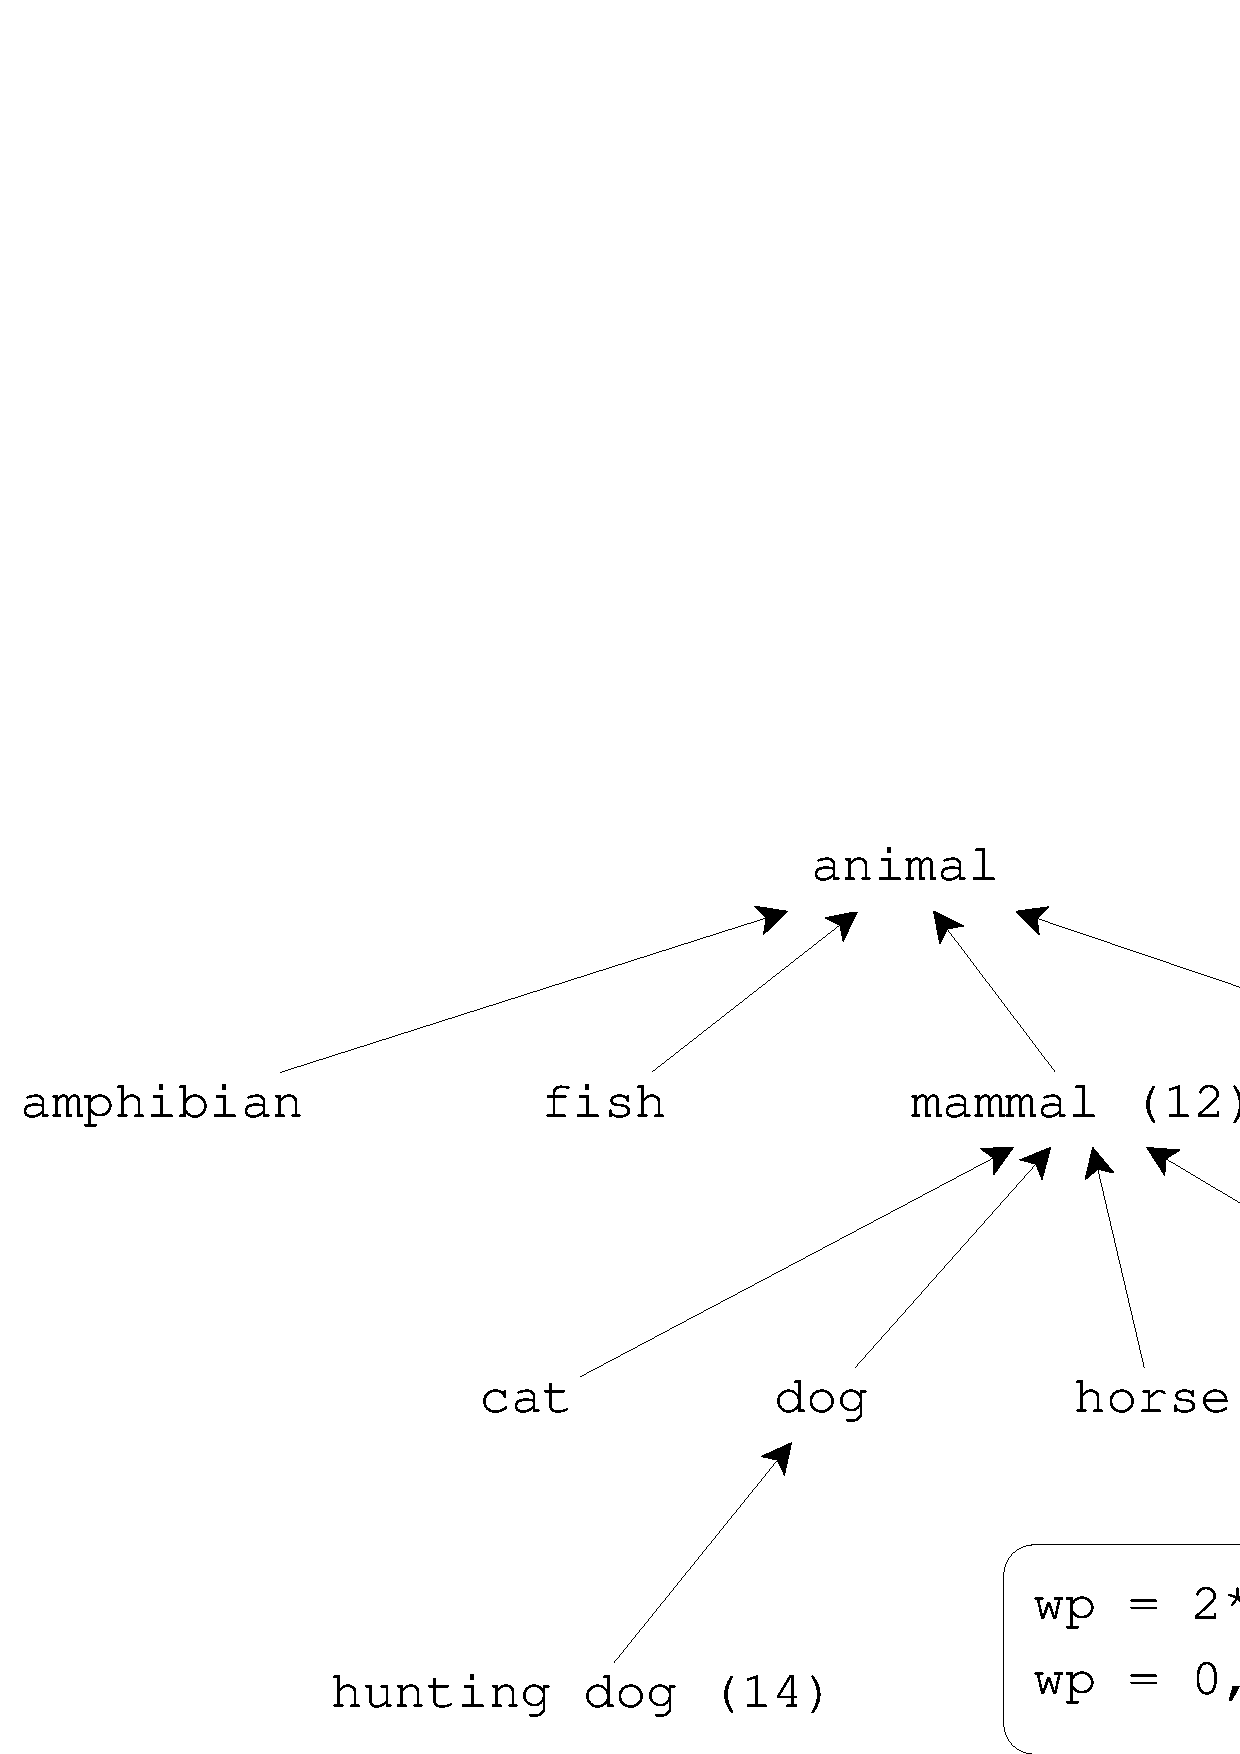
\includegraphics[width=0.8\linewidth]{fig-002.png}
    \caption{Posição dos anúncios nos primeiros resultados do Google.}
    \label{fig2}
    \source{Dados da pesquisa – coletados dos respondentes}
\end{figure}

O estudo de \textcite{rosa_publicidade_2022} reforça a ideia de que a maioria dos usuários entende que os anúncios nos resultados de pesquisa são personalizados e apresentados com base em seus interesses, entretanto, possuem conhecimentos mínimos acerca da personalização desses interesses.

Desse modo, apesar de haver certa ciência na forma como esses anúncios aparecem, e considerando que os resultados orgânicos e pagos são diferenciados visualmente pela plataforma, para o usuário que anseia por uma informação, um resultado é um resultado. Portanto, essa diferenciação pode passar despercebida. Questão essa que envolve vários aspectos acerca de como a informação é organizada e apresentada ao usuário na \textit{web}.

\textcite{camossi_conceito_2023} discutem questões relacionadas a técnicas de SEO no que diz respeito ao processo de ranqueamento dos resultados apresentados pelos mecanismos de busca, o que, nesse caso, está atrelado também aos anúncios dispostos junto aos resultados orgânicos.

\section{Operadores de pesquisa}\label{sec-fmt-manuscrito}
Operadores de pesquisa são caracteres especiais que, ao serem adicionados a uma expressão de busca, permitem criar uma maior complexidade a fim de obter resultados mais precisos. Em tese, um sistema de recuperação da informação pode transformar qualquer palavra ou símbolo em um operador de pesquisa de acordo com uma finalidade específica de busca dentro do seu banco de dados. Os operadores apresentados são o AND, Aspas, filetype: e site: conforme o \Cref{tab01}.

\begin{table}[h!]
\centering
\begin{threeparttable}
\caption{Descrição e função dos operadores avançados selecionados.}
\label{tab01}
\begin{tabular}{p{4.0cm} p{8.0cm}}
\toprule
\textbf{OPERADOR} & \textbf{FUNÇÃO RESUMIDA} \\
 \midrule
AND & Unir dois ou mais termos a fim de recuperar resultados que representem uma intersecção entre eles \\
Aspas “ ” & Blindar termos compostos ou frases completas a fim de recuperar resultados com todos os termos na ordem exata em que são indicados \\
filetype: & Indicar ao mecanismo de busca o formato exato de arquivo que deseja \\
site: & Indicar ao mecanismo de busca o site exato no qual você quer ele busque e apresente resultados \\
\bottomrule
\end{tabular}
\source{Dados da pesquisa (2022).}
\end{threeparttable}
\end{table}

O \textit{AND} é um operador booleano que corresponde à intersecção de dois ou mais termos. Numa busca, serve para garantir que o sistema apresentará resultados que contenham obrigatoriamente todos os termos ou expressões ligadas por ele \cite{picalho_logica_2022}. No caso da expressão 'google \textbf{AND} bing \textbf{AND} duckduckgo', os resultados retornarão documentos que citam os três termos descritos.

As aspas “ ” podem ser utilizadas sempre que existir um termo composto, frase completa ou até mesmo um parágrafo todo de texto, desde que seja de interesse do usuário recuperar documentos que constem todos os termos exatamente na ordem nas quais foram informados. Termos compostos como por exemplo: auxiliar administrativo ou ciência da informação podem ser acrescidos de aspas “ ” antes do primeiro e depois do último caractere da expressão para que um mecanismo de busca entenda que a pesquisa requer que ele retorne resultados exatamente como as expressões pedem. O resultado compreenderá apenas aqueles que apresentarem a expressão completa e exatamente na ordem na qual foi apresentada.

O \textit{filetype:} é um operador utilizado para pesquisar documentos que estejam em um formato de arquivo específico. Por exemplo: PDF, DOC, SRT, XLS, MP3, PNG, entre inúmeros outros. É útil para evitar que documentos com uma extensão de arquivo diferente da requerida pelo usuário apareça entre os resultados e pode ser utilizado antes ou depois da expressão de busca, entretanto, pode haver variação na quantidade e apresentação de resultados.

No caso dos exemplos 'modelos de currículo filetype:doc' e 'filetype:doc modelo de currículo'. Tematicamente, os resultados em ambas as expressões são similares. O mecanismo de busca retornará modelos de currículo editáveis em Word já que o formato indicado para a extensão de arquivo requerida foi DOC.

O operador site: é utilizado para direcionar a pesquisa realizada dentro da caixa de pesquisa para apenas um site em específico. Todos os resultados apresentados na página do mecanismo de busca virão obrigatoriamente de dentro do site indicado.


\section{Metodologia}\label{sec-formato}
Adotou-se uma situação de controle representada pela busca normalizada (cenário 2) e outros três cenários (cenário 3, 4 e 5) com diferentes intervenções a fim de observar alterações a partir delas. Neste sentido, o cenário 1 representou uma ação de busca livre efetuada pelo respondente.

As variáveis independentes neste estudo foram os operadores de pesquisa \textit{AND}, aspas, \textit{site:} e \textit{filetype:} que pretendiam influenciar a variável dependente representada pelos resultados visualizados a partir das capturas de tela.

A seleção destes operadores obedeceu a adequação para complementar a expressão de busca criada a partir da narrativa de pesquisa e com base na experiência de um dos autores enquanto bibliotecário. Como a busca visava encontrar documentos, o foco dos operadores foi auxiliar na união das palavras-chave (\textit{AND} e aspas \textit{“ ”}), na definição do formato de arquivo (\textit{filetype:}) e na fonte de informação (\textit{site:}).


\subsection{Respondentes}\label{sec-modelo}
Os respondentes da pesquisa de campo foram convidados por meio de divulgação do link de acesso ao questionário em grupos de pesquisa e mídias sociais (Instagram e Facebook) do pesquisador.

Não foram impostos critérios relacionados ao perfil pessoal, como idade ou gênero, para qualificar os usuários como aptos a participarem da pesquisa. Os pré-requisitos foram que o respondente tivesse acesso a um dispositivo com conexão à internet (\textit{smartphone}, \textit{tablet}, notebook ou computador de mesa) e possuísse uma conta no Gmail que estivesse ativa no momento das buscas e fosse informada para que o questionário pudesse ser respondido apenas uma vez.

\subsection{Procedimento}\label{sec-organizacao}
Foram desenvolvidos cinco testes de cenários de busca distintos, sendo que todos eles tratavam do mesmo tema: provas de concurso público para o cargo de auxiliar administrativo. A escolha ocorreu por conta da necessidade de criar uma busca fictícia que tivesse por objetivo a recuperação de algum tipo de documento na \textit{web}, neste caso, modelos de provas para um concurso público. O cargo de auxiliar administrativo foi definido por ser geralmente um cargo de nível médio, ampliando as possibilidades de resultados se comparado a cargos de nível superior.

Não era possível avançar para o próximo cenário sem antes ter realizado a atividade proposta pelo cenário anterior e cada seção juntamente com suas orientações era visualizada de forma única.

O cenário 1 (ver \Cref{fig3,fig4}) consistia em apresentar a temática ao respondente e instruí-lo a se imaginar na situação de uma pessoa interessada em encontrar provas de concurso públicos já realizados, para o cargo de auxiliar administrativo.

\begin{figure}[h!]
    \centering
    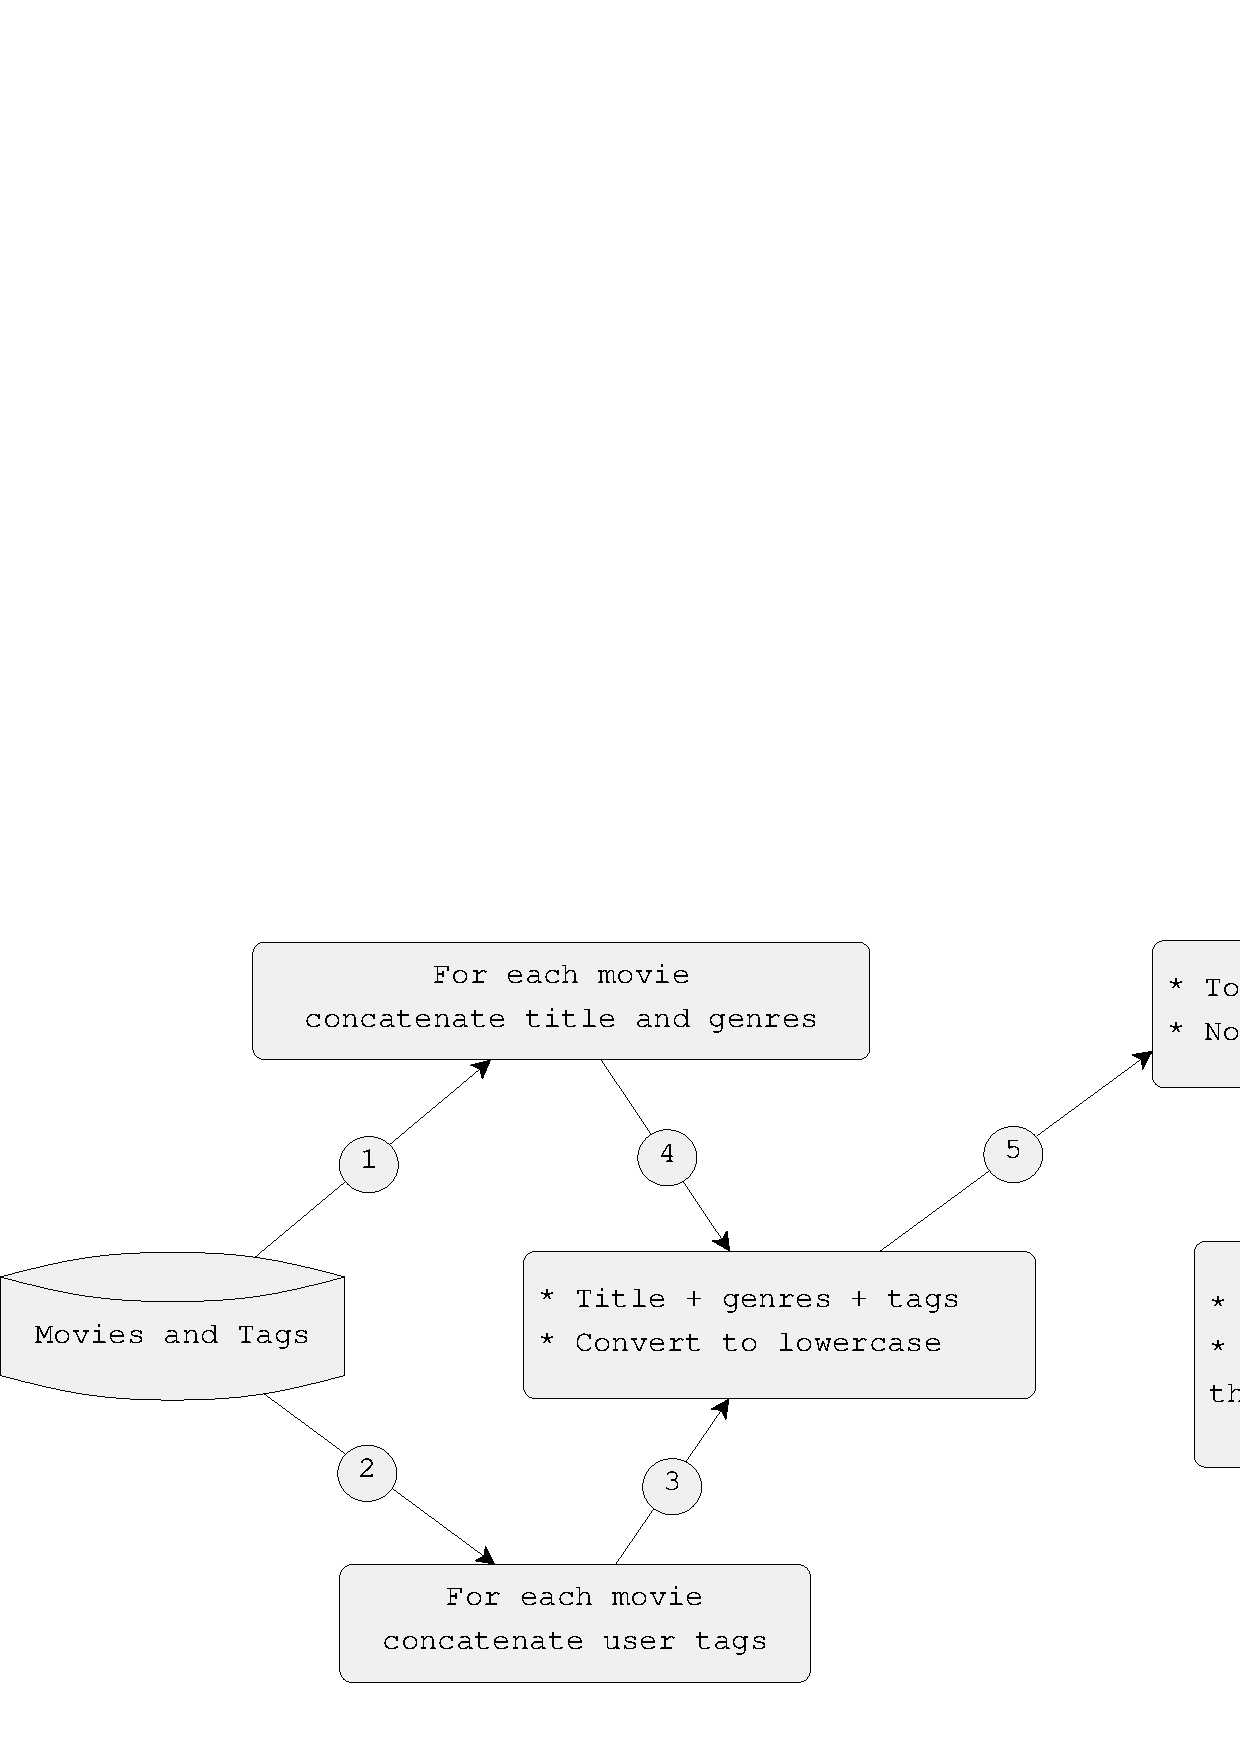
\includegraphics[width=0.8\linewidth]{fig-003.png}
    \caption{Cenário 1 do questionário de coleta de dados.}
    \label{fig3}
    \source{Dados da pesquisa – coletados dos respondentes}
\end{figure}

Nesse momento, o objetivo era coletar quais palavras-chave o usuário considerava relevantes e essenciais para realizar a busca diante do cenário apresentado. Foi solicitado que o usuário inserisse a expressão de busca executada em sua página do Google e realizasse o \textit{upload} da captura de tela com os resultados apresentados ao executá-la.

\begin{figure}[h!]
    \centering
    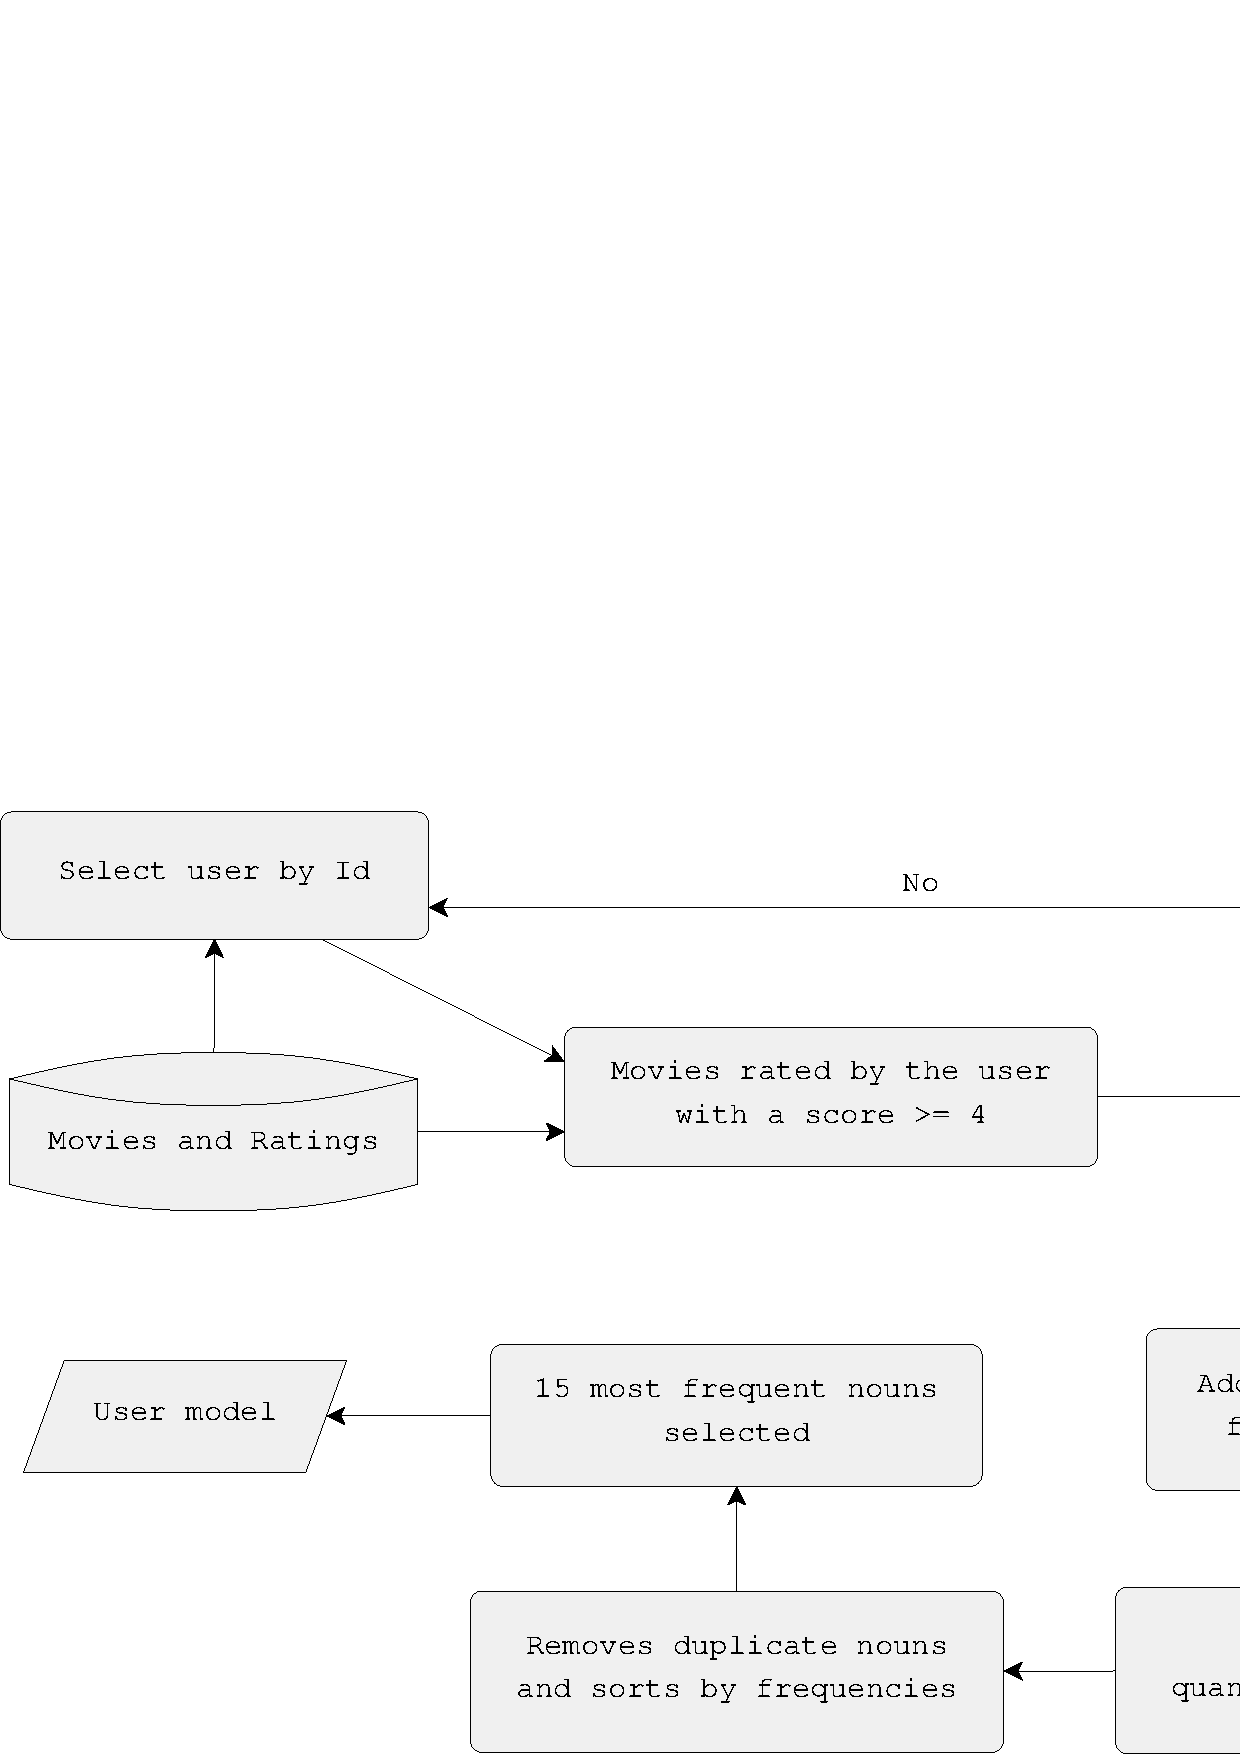
\includegraphics[width=0.8\linewidth]{fig-004.png}
    \caption{Campo de resposta do cenário 1.}
    \label{fig4}
    \source{Dados da pesquisa – coletados dos respondentes}
\end{figure}

Em todos os cenários foi orientado que o usuário realizasse a captura de tela sem considerar o aparecimento de anúncios, não sendo, portanto, necessário que ele rolasse a página de forma que só aparecessem resultados orgânicos em relação à busca realizada.

No cenário 2 da \Cref{fig5}, em vez de deixar a busca livre para que o usuário definisse as palavras-chave e a formulação das expressões de busca de acordo com seus próprios critérios, foi fornecida uma expressão única consolidada, para que ele copiasse, colasse em seu mecanismo de busca e executasse a pesquisa. A prática uniformizou a busca para todos os respondentes e teve por objetivos comparar os primeiros resultados de cada um deles.

\begin{figure}[h!]
    \centering
    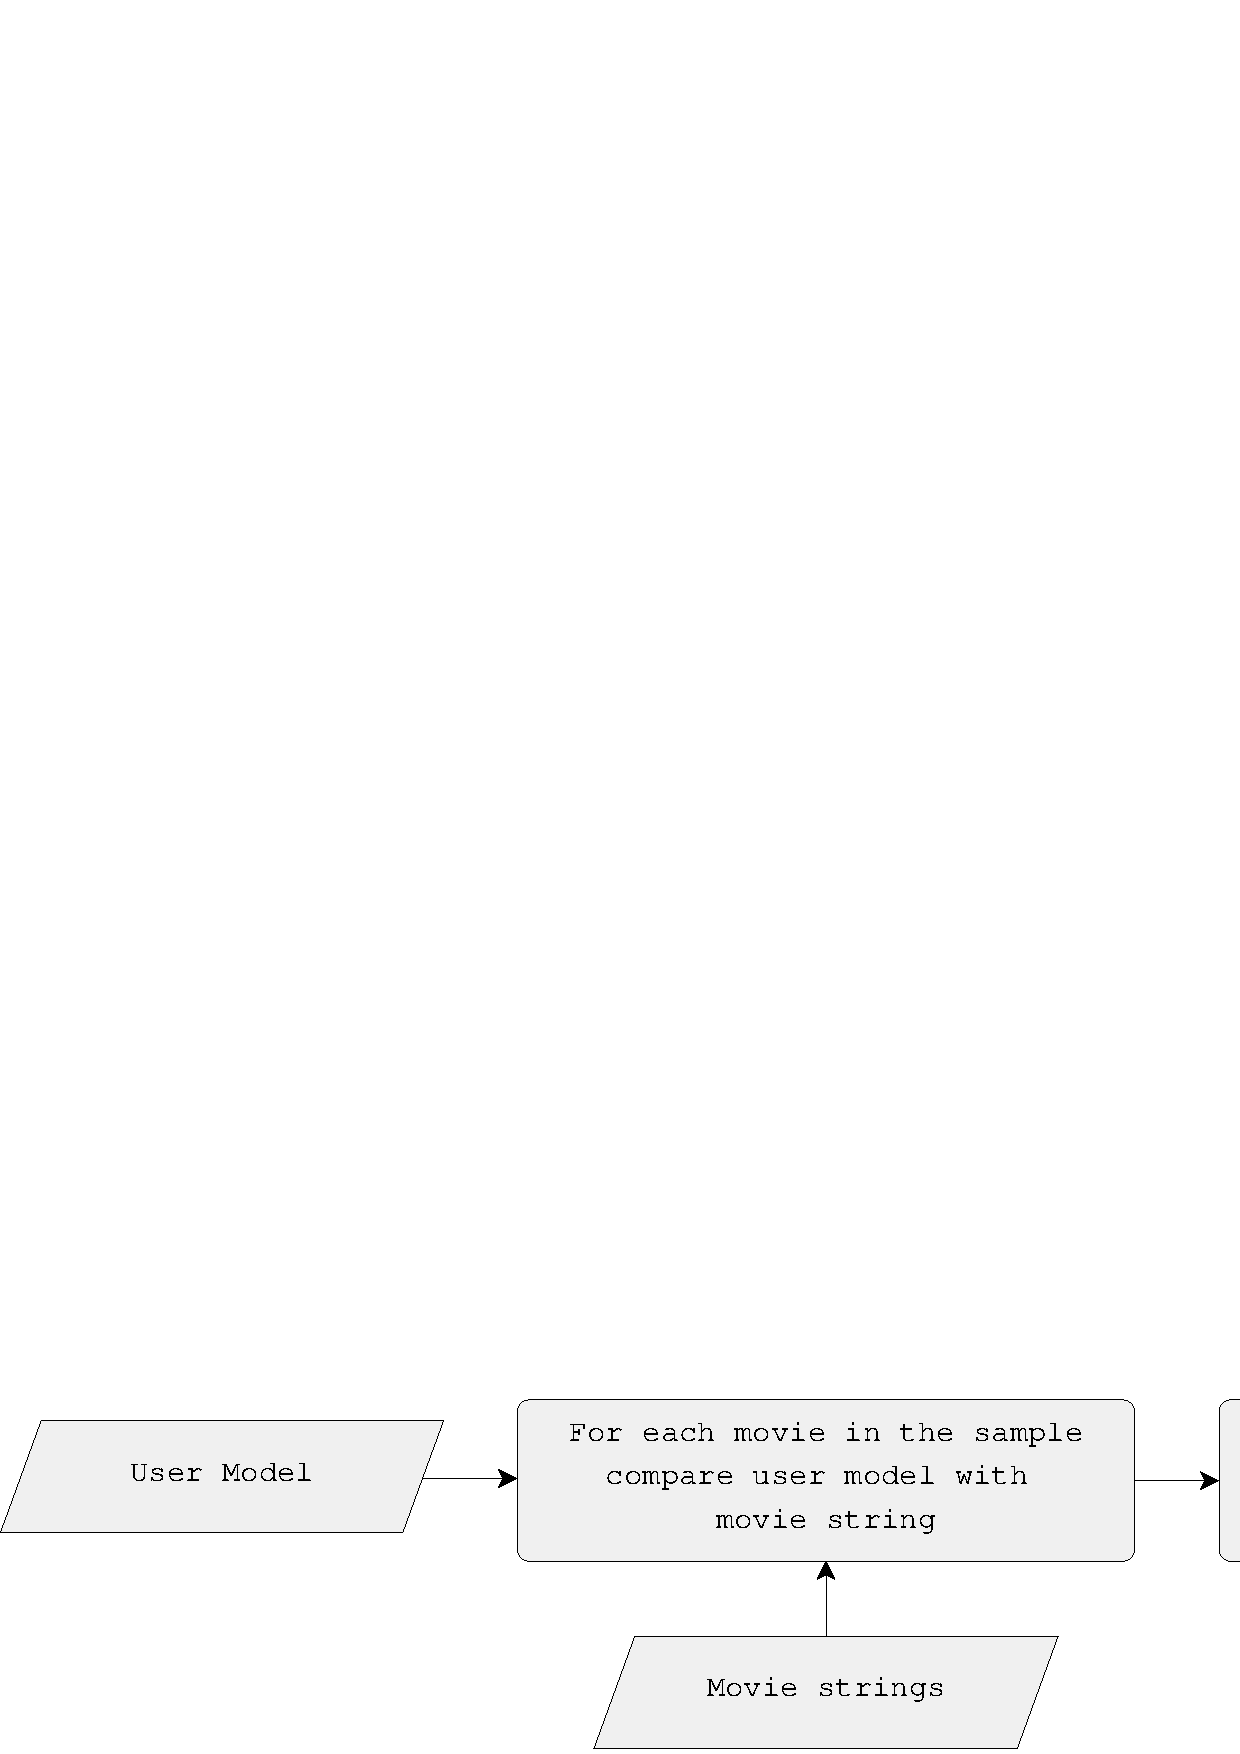
\includegraphics[width=0.8\linewidth]{fig-005.png}
    \caption{Cenário 2 do questionário de coleta de dados.}
    \label{fig5}
    \source{Dados da pesquisa – coletados dos respondentes}
\end{figure}

A partir do cenário 2, apenas a captura de tela era requerida ao respondente, e a forma de execução da pesquisa deveria vir acompanhada de um exemplo visual sobre como a caixa de pesquisa do Google deveria estar preenchida quando ele a realizasse.

O cenário 3 (ver \Cref{fig6}) introduz o uso de operadores ao determinar que o usuário utilizasse o operador booleano \textit{AND} na expressão de busca apresentada.

\begin{figure}[h!]
    \centering
    \includegraphics[width=0.8\linewidth]{fig-006.png}
    \caption{Cenário 3 do questionário de coleta de dados.}
    \label{fig6}
    \source{Dados da pesquisa – coletados dos respondentes}
\end{figure}

Mesmo que toda busca no Google de certa forma aplique o operador booleano \textit{AND} em sua execução, a ideia era testá-lo de forma mandatória, visando garantir somente resultados que obrigatoriamente apresentem as três expressões (\textit{concurso; auxiliar administrativo; provas}) juntas.

Além do uso do operador booleano \textit{AND}, nesse cenário, outro operador também foi empregado de forma combinada. As aspas \textit{“ ”}.

No cenário 4 (ver \Cref{fig7}) era requerido que os respondentes utilizassem o operador \textit{filetype:pdf} para que, ao aplicar a mesma pesquisa proposta pelos cenários 2 e 3, fossem restringidos os resultados para somente aqueles que apresentassem documentos de extensão no formato PDF (\textit{Portable Document Format}).

\begin{figure}[h!]
    \centering
    \includegraphics[width=0.7\linewidth]{fig-007.png}
    \caption{Cenário 4 do questionário de coleta de dados.}
    \label{fig7}
    \source{Dados da pesquisa – coletados dos respondentes}
\end{figure}

Ao utilizar o operador de formato \textit{filetype:} e restringir resultados apenas em PDF, esperava-se uma maior uniformização dos resultados nos diferentes perfis dos usuários respondentes do questionário.

Por último, o cenário 5 (ver \Cref{fig8}), introduziu o operador site: para que a mesma pesquisa reproduzida nos três cenários anteriores estivesse direcionada para resultados que viessem de um único \textit{site}.

\begin{figure}[h!]
    \centering
    \includegraphics[width=0.7\linewidth]{fig-008.png}
    \caption{Cenário 5 do questionário de coleta de dados.}
    \label{fig8}
    \source{Dados da pesquisa – coletados dos respondentes.}
\end{figure}

A escolha do \textit{site} utilizado ocorreu ao levar em consideração a preferência por uma banca de concursos que atuasse com provas para cargos de nível médio, em que o cargo de auxiliar administrativo estivesse presente. A banca selecionada para o exemplo da expressão de busca com o uso do operador foi o Instituto Quadrix. A organização sem fins lucrativos desenvolve e aplica provas para Conselhos Federais, Conselhos Regionais, Hospitais e Fundações, nos quais o cargo é recorrente, além de estar presente com atuação em todo Brasil, assegurando a abrangência nacional e variedade que o exemplo necessitava.

O cenário 5 apresentou o maior nível de especificidade na aplicação de operadores de pesquisa, restringindo mais ainda os resultados apresentados aos diferentes usuários respondentes do questionário.

\subsection{Coleta de dados}\label{sec-organizacao-latex}
O questionário foi construído na plataforma Google Forms e aplicado no segundo semestre de 2022. Ao todo, obteve um total de 76 respostas registradas durante o período.

A \Cref{tab02} resume a quantidade de capturas de tela que foram excluídas e quantas compuseram o total de cada cenário de busca descrito.

\begin{table}[h!]
\centering
\begin{threeparttable}
\caption{Conjunto de dados pré e pós-seleção.}
\label{tab02}
\begin{tabular}{l l l l}
\toprule
 \textbf{CENÁRIO DE BUSCA} & \textbf{COLETADOS} & \textbf{EXCLUÍDOS} & \textbf{ANALISADOS} \\
 \midrule
Busca livre & 76 & 00 & 76 \\
Busca normalizada & 76 & 04 & 72 \\
Operador booleano AND & 76 & 05 & 71 \\
Operador filetype: & 76 & 04 & 72 \\
Operador site: & 76 & 03 & 73 \\
\textbf{TOTAL} & 380 & 16 & 364 \\
\bottomrule
\end{tabular}
\source{Dados da pesquisa (2022).}
\end{threeparttable}
\end{table}

Cada respondente enviou cinco arquivos de imagem resultando num total de 380 capturas de tela coletadas. Destes, 16 não puderam ser analisadas. A exclusão ocorreu por problemas como: captura da tela não correspondente ao solicitado, expressão de busca formulada incorretamente ou pesquisa realizada em outro mecanismo de busca diferente do solicitado. Assim sendo, o \textit{corpus} da pesquisa analisado resultou em 364 capturas de tela.

\section{Contribuições para a ciência aberta}\label{sec-titulo}
Para \textcite[p. 17]{lecardelli_dados_2020} “compartilhar informações científicas é primordial para potencializar os avanços da ciência, poupar retrabalho, possibilitar reproduzir pesquisas para validação e permitir o reuso de informações por novos interessados para novas descobertas”. Portanto, se tem como compromisso, neste trabalho, contribuir para a ciência aberta, permitindo a disponibilização dos dados científicos gerados no desenvolvimento da pesquisa.

Em conformidade com a Lei Geral de Proteção de Dados (LGPD) em relação ao tratamento de dados em território nacional, todas as 380 capturas de tela foram anonimizadas, fotos de perfil, nomes de usuário e outras guias abertas no navegador foram anuladas. Além disso, os arquivos de imagem tiveram seus metadados relacionados a propriedade e informações pessoais foram removidas.

As planilhas criadas a partir das capturas de tela coletadas foram disponibilizadas no repositório de dados científicos abertos Zenodo, mantido pela \textit{European Organization for Nuclear Research} (CERN). A escolha foi realizada por conta da possibilidade de depósito gratuito dos dados por parte dos autores, acrescida da atribuição do identificador persistente \textit{Digital Object Identifier} (DOI) que concede singularidade e permanência a objetos digitais na internet.

Dito isso, os dados abertos desta pesquisa encontram-se disponíveis em: \url{https://doi.org/10.5281/zenodo.7434768}.

\section{Análise dos resultados}\label{sec-autores}
Os dados geográficos demonstraram que 93\% dos respondentes estavam em alguma localidade do Brasil no momento de preenchimento do questionário, e 7\% estavam em outros países, sendo eles: Portugal, Colômbia, Argentina e Canadá.

Dos que estavam no Brasil, o Sul apresentou maior incidência com 69\% do total. Seguido pelo Sudeste com 22\%. As demais regiões Nordeste, Centro Oeste e Norte ficaram com 6\%, 3\% e 0\%, respectivamente (ver \Cref{fig9}).

\begin{figure}[h!]
    \centering
    \includegraphics[width=0.8\linewidth]{gra-001.pdf}
    \caption{Dados de geolocalização dos respondentes.}
    \label{fig9}
    \source{Dados da pesquisa (2022).}
\end{figure}

Em relação ao tipo de dispositivo que foi utilizado pelos respondentes para completar o questionário, a divisão ficou em 55\% para notebook ou computador de mesa e 45\% para smartphone (ver \Cref{fig10}). Nenhum respondente utilizou tablet para completar a pesquisa.

\begin{figure}[h!]
    \centering
    \includegraphics[width=0.8\linewidth]{gra-002.pdf}
    \caption{Tipo de dispositivo utilizado pelos respondentes.}
    \label{fig10}
    \source{Dados da pesquisa (2022).}
\end{figure}

A maioria respondeu ao questionário por meio do navegador Google Chrome, representando 78\% do total. Para os demais, 11\% utilizaram o Safari, 5\% o Mozilla Firefox, 3\% o Opera. Microsoft Edge, Brave Browser e Samsung Internet atingiram 1\% cada (ver \Cref{fig11}).

\begin{figure}[h!]
    \centering
    \includegraphics[width=0.8\linewidth]{gra-003.pdf}
    \caption{Navegador de internet utilizado pelos respondentes.}
    \label{fig11}
    \source{Dados da pesquisa (2022).}
\end{figure}

Outro dado coletado foi acerca da utilização ou não de bloqueadores de anúncios nos navegadores utilizados durante o preenchimento do questionário (ver \Cref{fig12}).

\begin{figure}[h!]
    \centering
    \includegraphics[width=0.8\linewidth]{gra-004.pdf}
    \caption{Presença de bloqueador de anúncios no navegador.}
    \label{fig12}
    \source{Dados da pesquisa (2022).}
\end{figure}

De modo geral, 8\% dos respondentes afirmaram não utilizar nenhum tipo de bloqueador de anúncio, enquanto 17\% que utilizam ou não souberam responder, sendo essa última parcela distribuída em 13\% para o uso do \textit{AdBlock}, 1\% para o \textit{uBlock} e 3\% não souberam responder por dúvidas se essa é uma ferramenta que estava instalada em seu navegador de forma automática ou por terceiros sem que eles soubessem.

\subsection{Busca livre}\label{sec-idioma}
A busca livre corresponde ao cenário 1, considerando a narrativa apresentada no questionário para que o usuário realizasse a pesquisa livremente. Portanto, o primeiro resultado diz respeito às escolhas dos termos efetuadas por cada respondente (ver exemplo \Cref{fig13}).

O cenário 1 solicitava se imaginar na situação de uma pessoa interessada em encontrar provas de concurso públicos já realizados, para o cargo de auxiliar administrativo.

\begin{figure}[h!]
    \centering
    \includegraphics[width=0.8\linewidth]{fig-009.png}
    \caption{Execução da busca livre.}
    \label{fig13}
    \source{Dados da pesquisa – coletado dos respondentes (2022).}
\end{figure}

Os três termos com maior ocorrência na expressão de busca livre criada pelos respondentes foram \textit{auxiliar administrativo} com 69 usos (91\% dos usuários), seguido de \textit{prova} com 63 (83\% dos usuários) e concurso com 59 (78\% dos usuários). Sem levar em consideração: plurais e variações, ainda assim os três termos citados continuam com maior ocorrência dentro das pesquisas, nessa mesma ordem.

A maioria dos respondentes entendeu a busca livre da mesma forma que a busca normalizada. Isto é, grande parte dos respondentes utilizou os mesmos termos empregados posteriormente na busca com termos pré-indicados.

Além disso, também é possível notar o acréscimo de outros termos complementares à expressão de busca na nuvem de palavras da \Cref{fig14}. Ao todo, 55\% dos usuários utilizaram algum termo adicional em relação aos três principais citados. Desses, apenas 12\% empregaram algum tipo de operador avançado por conhecimento próprio.

\begin{figure}[h!]
    \centering
    \includegraphics[width=0.8\linewidth]{fig-010.png}
    \caption{Nuvem de palavras com os termos da busca livre.}
    \label{fig14}
    \source{Dados da pesquisa (2022).}
\end{figure}

As \textit{stop words}\footnote{\textit{Stop words} ou palavras-vazias são termos que possuem pouco significado num contexto tais como preposições, artigos, conjunções e outras \cite{ibict_stop_2015}.} não foram ignoradas, pois fazem sentido diante do contexto. Mesmo sendo palavras consideradas pela computação como vazias e com uma função semântica praticamente irrelevante para a lógica de indexação e apresentação do conjunto de resultados pelos mecanismos de busca, as \textit{stop words} foram mantidas com intuito de representar a necessidade sentida pelos respondentes em inseri-las na sua expressão de busca livre.

Contradizendo a questão da total irrelevância dos resultados e tendo por base a observação das capturas de tela coletadas neste cenário, principalmente no que diz respeito a quantidade e ordem dos resultados, toda preposição, conjunção ou até um caractere a mais na expressão de busca, fez diferença (mesmo que não contextualmente) para o mecanismo de busca. Consequentemente, apresentou resultados diferentes daqueles sem tais acréscimos. Uma busca que utilizou a expressão \textit{provas concurso público} apresentou resultados diferentes de uma pesquisa como \textit{provas de concursos público} e, ainda diferentes, de uma pesquisa como \textit{prova de concurso público}, mesmo que a diferença seja apenas um acento agudo.

Em relação ao aspecto visual, os tamanhos representam a frequência com que os termos apareceram. As cores dividem os termos em sete categorias: a cor azul petróleo (\raise.75ex\hbox{\colorbox{teal!70}{   }}) refere-se aos termos relacionados ao cargo em questão; a cor roxa (\raise.75ex\hbox{\colorbox{violet!70}{   }}) para termos relacionados ao documento; a cor vermelha (\raise.75ex\hbox{\colorbox{red!70}{   }}) para termos relacionados ao evento; a cor marrom (\raise.75ex\hbox{\colorbox{brown!100!}{   }}) para termos de ligação; a cor verde (\raise.75ex\hbox{\colorbox{blue!20!black!30!green}{   }}) para outros termos relacionados; a cor rosa (\raise.75ex\hbox{\colorbox{magenta!70}{   }})  para operadores de pesquisa avançados e a cor cinza (\raise.75ex\hbox{\colorbox{gray!70}{   }}) para sinais ortográficos. O grau de opacidade de cada uma delas corresponde à importância dentro da categoria pertencente. Todas as cores foram escolhidas aleatoriamente.

Consequentemente, a partir de uma busca livre, os resultados são diversificados, e como já dito, cada acento, plural ou qualquer outro caractere, pode conduzir a resultados diferentes.

\subsection{Busca normalizada}\label{sec-resumo}
O cenário 2 apresentou uma busca pronta designada como: concurso auxiliar administrativo provas e solicitou que o respondente a replicasse em sua própria caixa de pesquisa (ver exemplo \Cref{fig15}).

\begin{figure}[h!]
    \centering
    \includegraphics[width=0.8\linewidth]{fig-011.png}
    \caption{Execução da busca normalizada.}
    \label{fig15}
    \source{Dados da pesquisa – coletado dos respondentes (2022).}
\end{figure}

A busca normalizada apresentou resultados mais uniformes que a busca livre. Das 72 capturas de telas válidas analisadas, os resultados em notebooks ou computadores de mesa variaram entre aproximadamente 5.500.000 e 8.000.000 de resultados recuperados. Apenas uma busca teve 34.100.000 links, sendo que o usuário estava no Brasil e informou utilizar um bloqueador de anúncios no navegador Google Chrome.

Em apenas seis capturas de tela notou-se a presença de propagandas no topo dos resultados orgânicos. Esses 8\% do total da categoria foram pesquisados utilizando o navegador Google Chrome. Nenhum deles apresentou sugestões de outras pesquisas realizadas no tema, que estavam presentes em outros 83\% das capturas de tela, todas sem publicidade. Sugere-se uma relação entre a presença de publicidade e o aparecimento de recomendações de outras pesquisas já realizadas. No entanto, os demais cenários não confirmaram tal hipótese se comparada a pesquisas com o uso de operadores avançados, já que os cenários 2, 3 e 4 tiveram pesquisas que apresentaram publicidade juntamente com sugestões de pesquisas feitas por outros usuários e não apresentaram dados suficientes para comprovar uma correlação entre esses dois tópicos.

\subsection{Busca com o operador booleano \textit{AND}}\label{sec-secoes}
O cenário 3 foi o primeiro a acrescentar um operador de pesquisa e apresentou uma expressão de busca com o uso do \textit{AND}. O operador booleano funcionou com apenas seis respondentes de um total de 71. Isto porque para 65 usuários, a expressão de busca foi alterada pelo sistema. A alteração substituiu o primeiro booleano \textit{AND} pela preposição \textit{DE} como é possível verificar na \Cref{fig16}.

\begin{figure}[h!]
    \centering
    \includegraphics[width=0.8\linewidth]{fig-012.jpg}
    \caption{Erro de pesquisa com o operador booleano \textit{AND}.}
    \label{fig16}
    \source{Dados da pesquisa – coletado dos respondentes (2022).}
\end{figure}

O mecanismo de busca considera todas as pesquisas realizadas com mais de um termo como já acrescidas do operador booleano \textit{AND} em sua expressão. Portanto, um usuário que pesquisa por ‘provas concurso auxiliar administrativo’ já tem todos esses quatro termos multiplicados logicamente em decorrência do operador.

Em vista disso, entende-se que nesse caso o sistema realizou uma correção textual ao não interpretar o \textit{AND} como um operador e sim como mais um termo de busca de valor textual semelhante aos termos ‘concurso’ ou ‘provas’, por exemplo. Como o objetivo era avaliar a efetividade do booleano com diferentes usuários numa mesma busca e não o conhecimento sobre o buscador e possíveis ações corretivas, a orientação foi que a captura de tela fosse registrada sem nenhuma interferência do usuário, que poderia informar ao mecanismo de busca para não efetuar a troca e refazer a pesquisa da forma proposta inicialmente.

As pesquisas em que o booleano foi aceito pelo mecanismo de busca não apresentaram os avisos da \Cref{fig16} e tiveram resultados exibidos normalmente conforme a \Cref{fig17}.

\begin{figure}[h!]
    \centering
    \includegraphics[width=0.8\linewidth]{fig-013.png}
    \caption{Pesquisa bem-sucedida com o operador booleano \textit{AND}.}
    \label{fig17}
    \source{Dados da pesquisa – coletado dos respondentes (2022).}
\end{figure}

Após análise, ao que parece, somente cinco usuários tiveram suas pesquisas validadas pelo mecanismo de busca como uma pesquisa que requer ao sistema o uso forçado e explícito do operador booleano \textit{AND} por duas vezes. As cinco pesquisas não apresentaram nenhum anúncio no topo ou ao lado dos primeiros resultados, sendo que nenhum deles afirmou estar utilizando um bloqueador de anúncios.

Todas as cinco, ainda que o mecanismo de busca tenha executado a expressão, foram questionadas pelo sistema se a pesquisa de fato era a que foi informada ou se a intenção era a pesquisa concurso DE “\textit{auxiliar administrativo}” \textit{AND provas}, executada automaticamente pela grande maioria dos respondentes dessa categoria.

Das seis capturas de tela excluídas da categoria, duas delas, a princípio, pareciam ter o operador booleano executado corretamente. No entanto, o número de resultados aproximados ficou aquém do esperado para uma expressão de busca tão específica, ambos acima de 350 mil. Outro ponto percebido foi que duas dessas capturas de tela estavam relacionadas a mecanismos de busca configurados em outros idiomas que não o português brasileiro, uma delas estava em inglês e outra em espanhol.

Levando em consideração que das buscas válidas, apenas 7\% obtiveram êxito, sugere-se que, para a maioria dos usuários, o operador \textit{AND} não tende a funcionar de início em buscas com apenas um termo composto acrescido de aspas junto a outros dois termos únicos. Entretanto, funciona implicitamente por ser um parâmetro empregado em todas as buscas com vários termos.

Como se trata de uma função que já ocorre logicamente em toda pesquisa realizada no sistema, ao acessar a aba de pesquisa avançada do Google, somente outros operadores booleanos com o OR e o NOT são disponibilizados aos usuários, conforme a \Cref{fig18}.

\begin{figure}[h!]
    \centering
    \includegraphics[width=0.8\linewidth]{fig-014.png}
    \caption{Guia de pesquisa avançada do Google.}
    \label{fig18}
    \source{\cite{google_uncios_2022}}
\end{figure}

O mecanismo de busca permite localizar resultados que contenham qualquer uma das palavras, usando o \textit{OR} e com nenhuma das palavras citadas, utilizando o \textit{NOT}, na forma de ‘–‘ (sinal de menos).

\subsection{Busca com o operador avançado \textit{filetype:}}\label{sec-format-simple}
O cenário 4 apresentou o operador avançado \textit{filetype:} com foco em obter precisão nos formatos dos documentos recuperados. A expressão de busca com o uso de operador \textit{filetype:} funcionou com 70 respondentes do total de 72 válidos. Dos excluídos, um apresentou a mensagem de que houve resultados que coincidiram com a expressão pesquisada, no entanto, o operador de pesquisa precisaria ser incluído naquele resultado em si, o que denota que o sistema o interpretou como um termo simples e não um comando de busca avançado como é possível observar na \Cref{fig19}.

\begin{figure}[h!]
    \centering
    \includegraphics[width=0.5\linewidth]{fig-015.png}
    \caption{Erro no uso do operador \textit{filetype:}.}
    \label{fig19}
    \source{Dados da pesquisa – coletados dos respondentes (2022).}
\end{figure}

Neste caso, o usuário não especificou o formato de arquivo requerido e indicado no questionário, que no caso era PDF. Qualquer outra extensão de arquivo, caso fosse especificada, não seria listada pelo mecanismo de busca como possível inclusão de termo já que ele entenderia como um comando direto mesmo que o resultado fosse zero arquivos recuperados.

Nas 70 demais buscas é possível observar uma etiqueta após a URL de cada resultado, confirmando que o documento hospedado naquele site é na extensão requerida na expressão de busca, no caso, PDF (ver \Cref{fig20}).

\begin{figure}[h!]
    \centering
    \includegraphics[width=0.6\linewidth]{fig-016.png}
    \caption{Etiqueta com extensão de arquivo.}
    \label{fig20}
    \source{Dados da pesquisa – coletados dos respondentes (2022).}
\end{figure}

Em geral, também é possível afirmar que, para a amostra analisada, o operador não influenciou na aparição ou não de anúncios e suas respectivas posições em tela ou sugestões de pesquisas. Em relação a quantidade aproximada de resultados em pesquisas realizadas em \textit{notebooks} ou computadores de mesa foi mantida a variação entre 1.000.000 e 1.600.00 de resultados. Apenas dois destoaram desse número, um para mais e outro para menos, o que é justificado pela geolocalização dos dois usuários que estavam fora do Brasil no momento das buscas.

\subsection{Busca com o operador avançado \textit{site:}}\label{sec-links}
O cenário 5 contava com o uso do operador \textit{site:} a fim de especificar ao mecanismo de busca a fonte principal de informação dos resultados a serem apresentados. Os resultados mostram que o operador site: funcionou nas 73 capturas de tela válidas analisadas dentro da categoria.

Com o operador avançado \textit{site:} foi possível observar o maior nível de similaridade entre os primeiros resultados e as perguntas sugeridas pelo próprio mecanismo de busca como pesquisas similares que outros usuários realizaram.

Em relação aos anúncios, este foi o operador que mais influenciou na presença de publicidade dentre os resultados. De todas as 73, somente uma apresentou um anúncio no topo, o que gerou controvérsias tendo em vista que o usuário em questão afirmou utilizar um bloqueador de anúncios em seu navegador (ver \Cref{fig21}).

\begin{figure}[h!]
    \centering
    \includegraphics[width=0.6\linewidth]{fig-017.jpg}
    \caption{Etiqueta com extensão de arquivo.}
    \label{fig21}
    \source{Dados da pesquisa – coletados dos respondentes (2022).}
\end{figure}

Esse mesmo respondente que indicou o utilizar bloqueadores de anúncios, também apresentou outra captura de tela com a presença de anúncios na categoria do operador \textit{filetype:}. Nesse caso, ou a informação cedida por ele em relação ao uso de um bloqueador de anúncios estava incorreta ou o funcionamento deste bloqueador foi comprometido em níveis mais avançados de busca com a presença de operadores como \textit{filetype:} e \textit{site:}.

A quantidade aproximada de resultados em pesquisas realizadas em \textit{notebooks} ou computadores de mesa variou entre 900 e 2300 resultados, sendo, portanto, o operador que mais trouxe exatidão aos resultados, retornando para o usuário um número consideravelmente baixo em comparação aos outros quatro cenários nos quais havia resultados na casa dos milhões. Ocorrência que condiz com a funcionalidade do operador, já que seu uso permite apontar somente para resultados advindos de uma única fonte. Nesse caso, a quantia é relativa, mas a fonte de busca é precisa.

\subsection{Observações gerais}\label{sec-outras-estr}
Em 10 das 380 capturas de tela, os respondentes, por conta própria, rolaram a tela e realizaram a ação. Algumas imagens trazem apenas resultados abaixo da caixa de pesquisa, o que leva a crer que anúncios foram ignorados e desconsiderados pelos respondentes como resultados válidos frente a expressão de busca pesquisada.

Em oito capturas de tela, mesmo os usuários que informaram utilizar um bloqueador de anúncios, tiveram anúncios exibidos em suas pesquisas. Seis deles ao utilizarem o operador \textit{filetype:}. O uso dos bloqueadores não interferiu na quantidade de resultados aproximados informada pelo mecanismo de busca em comparação aos que não utilizaram.

Os diferentes navegadores, bem como o uso de \textit{smartphones} ou \textit{notebooks} e computadores de mesa, não manifestaram características que visivelmente interferissem no uso de funcionamento dos operadores propostos na pesquisa.

As características que mais se destacaram nas buscas foram a presença de anúncios, sugestões de outras pesquisas já realizadas que tinham relação com a pesquisa atual e resultados aproximados em \textit{notebooks} ou computadores de mesa.

Em relação a presença de anúncios no topo dos resultados, calculou-se a porcentagem de pesquisas que apresentaram anúncios dentre os respondentes que informaram não utilizar nenhum tipo de bloqueador de anúncios (ver \Cref{tab03}).

\begin{table}[h!]
\centering
\begin{threeparttable}
\caption{Porcentagem de anúncios nos cenários normalizados.}
\label{tab03}
\begin{tabular}{l l}
\toprule
 \textbf{CENÁRIO DE BUSCA} & \textbf{ANÚNCIOS} \\
 \midrule
Busca normalizada & 9\% \\
Busca com o AND e as aspas & 0\% \\
Busca com o filetype: & 39\% \\
Busca com o site: & 2\% \\
\bottomrule
\end{tabular}
\source{Dados da pesquisa (2022).}
\end{threeparttable}
\end{table}

Nota-se que uso de alguns operadores avançados pode favorecer a aparição de anúncios de pesquisa à medida que ou obrigatoriamente o anunciante tenha usado todas as palavras-chave da intersecção resultante do uso do operador booleano \textit{AND} acrescido as aspas, ou esteja atrelado ao \textit{site} indicado como fonte única de pesquisa do operador \textit{site:}.

Se a busca realizada pelo operador \textit{filetype:} indicar um formato de arquivo atrelado ao produto anunciado, existe a possibilidade deste produto se encaixar nos resultados como anúncio de pesquisa (ver \Cref{fig22}). Isso está atrelado a personalização descrita no estudo de \textcite{rosa_publicidade_2022} e as técnicas de SEO empregadas na indexação de conteúdos web, exploradas no estudo de \textcite{camossi_conceito_2023}.

\begin{figure}[h!]
    \centering
    \includegraphics[width=0.8\linewidth]{fig-018.jpg}
    \caption{Anúncios de apostilas usando o operador \textit{filetype:}.}
    \label{fig22}
    \source{Dados da pesquisa – coletados dos respondentes (2022).}
\end{figure}

Nos dados coletados, o formato PDF sempre esteve ligado a anúncios de apostilas, provavelmente comercializada nesse formato de arquivo. Na sequência, calculou-se a porcentagem das capturas de tela em que as sugestões de pesquisa apareciam dentro dos cenários normalizados (ver \Cref{tab04}).

\begin{table}[h!]
\centering
\begin{threeparttable}
\caption{Porcentagem das sugestões de pesquisa nos cenários normalizados.}
\label{tab04}
\begin{tabular}{l l}
\toprule
 \textbf{CENÁRIO DE BUSCA} & \textbf{SUGESTÕES} \\
 \midrule
Busca normalizada & 83\% \\
Busca com o AND e as aspas & 100\% \\
Busca com o filetype: & 76\% \\
Busca com o site: & 92\% \\
\bottomrule
\end{tabular}
\source{Dados da pesquisa (2022).}
\end{threeparttable}
\end{table}

Não houve uma grande variação que possa inferir correlação entre o aparecimento ou não de sugestões (ver \Cref{fig23}) a partir do uso dos operadores avançados testados. No entanto, as sugestões quase sempre presentes, corroboram o dito por \textcite{santos_avaliacao_2015} ao trazer a ideia de que encontrar resultados satisfatórios para uma pesquisa, levará a produção de novos conhecimentos, que são disponibilizados na web e consequentemente atrelados às pesquisas que o precederam, como as sugestões.

\begin{figure}[h!]
    \centering
    \includegraphics[width=0.8\linewidth]{fig-019.png}
    \caption{Exemplo de sugestões de pesquisas já realizadas.}
    \label{fig23}
    \source{Dados da pesquisa – coletados dos respondentes (2022).}
\end{figure}

Por fim, calculou-se a mediana entre as pesquisas realizadas em notebooks e computadores de mesas, no que diz respeito à quantidade de resultados aproximados (ver \Cref{tab05}).

\begin{table}[h!]
\centering
\begin{threeparttable}
\caption{Mediana dos resultados nos cenários normalizados.}
\label{tab05}
\begin{tabular}{l l}
\toprule
 \textbf{CENÁRIO DE BUSCA} & \textbf{MEDIANA DOS RESULTADOS APROXIMADOS} \\
 \midrule
Busca normalizada & 7.400.000 \\
Busca com o AND e as aspas & 4 \\
Busca com o \textbf{filetype:} & 1.270.000 \\
Busca com o \textbf{site:} & 1.930 \\
\bottomrule
\end{tabular}
\source{Dados da pesquisa (2022).}
\end{threeparttable}
\end{table}

Os resultados apontam para uma redução na quantidade total de resultados ao utilizar operadores avançados de pesquisa se comparado a uma busca sem eles. Afinal, quanto mais específica for a expressão, menor é a quantidade de documentos dentro do índice em que o mecanismo de busca realizará a varredura à procura de resultados precisos.

Essa possibilidade de aumentar a precisão dos resultados por meio do uso de operadores endossa a importância de conhecê-los e saber empregá-los quando preciso. Resultados como os apresentados por \textcite{mnguni_web_2022} trazem o Google como a ferramenta de busca mais utilizada por estudantes universitários para encontrar informações, sendo um público que necessita desses conhecimentos diante do volume de resultados apresentados em grande parte das pesquisas e como consequência da transformação do ato de pesquisar, proporcionada pelas tecnologias de informação e comunicação como os mecanismos de busca \cite{gonzalez_guitian_comportamiento_2022}.

\section{Considerações finais}\label{sec-listas}
Mecanismos de busca estão em constante aprimoramento para melhorar a experiência de pesquisa dos usuários. Muitas vezes a forma simples funciona, pois o usuário insere um ou mais termos, clica em buscar e navega pelos resultados apresentados em tela. Todavia, é importante conhecer recursos para que, caso venha a precisar, possa recorrer a estratégias específicas visando encontrar um conjunto menor ou mais padronizado de resultados para avaliar, fazendo com que tal tarefa possua mais assertividade e precisão. 	
O sucesso de um processo de busca na internet pode ser analisado desde a construção da expressão de busca — com ou sem o uso de operadores —, até o resultado apresentado em tela. Este resultado ainda pode apresentar elementos de \textit{feedback} que apontam sucesso ou fracasso daquilo que foi solicitado pelo usuário. Ou seja, se a expressão construída de fato foi entendida pelo mecanismo de busca e funcionou.

Diante disto, e após as observações realizadas neste trabalho, é possível apresentar duas reflexões. A primeira se refere ao \textit{funcionamento da expressão de busca}. Ao efetuar uma expressão de busca com operadores booleanos, e o retorno não apresentar resultados, pode-se imaginar que a expressão de busca não funcionou.

Porém, uma pesquisa retornar zero resultados não quer dizer que a expressão de busca estava incorreta. Ela pode ter funcionado sem nenhum erro de sintaxe e constatado que não há nada ali correspondendo ao que foi pesquisado.

Já num segundo cenário reflexivo, usa-se uma expressão de busca com operadores booleanos, e nesse caso, suponha que a pesquisa retornou com 23 resultados.

Essa segunda reflexão, é sobre a \textit{precisão dos resultados}. Uma pesquisa retornar resultados não quer dizer que a expressão de busca foi precisa. A depender da situação, alguns sistemas podem ignorar operadores ou retornar resultados com partes da expressão. Usuários mais desavisados podem achar que a expressão foi executada exatamente como ele construiu, quando na verdade o sistema usou outros caminhos para apresentar os resultados.

Esse último caso fica explícito nas pesquisas utilizando o operador booleano \textit{AND} que compuseram esse estudo. No caso, o mecanismo de busca informou que estava exibindo resultados para uma expressão de busca que não a solicitada. Contudo, nem sempre isso acontece e cabe sempre ao usuário examinar se aqueles resultados que retornaram equivalem a ideia inicial de expressão que ele elaborou e construiu.

Isto é importante e se relaciona com todo o processo de observações realizado neste trabalho à medida que tais operadores avançados não estão presentes na interface inicial da tela de busca e nem são apresentados aos usuários como sugestões. Assim, demandam que os usuários tenham um prévio conhecimento de como funcionam e para que servem, de modo a evitar um uso inadequado ou ineficaz dos operadores.

Das características nos resultados de pesquisa que se destacam a partir do uso de operadores avançados na busca por documentos na \textit{web} estão os anúncios de pesquisa, as sugestões de pesquisas que já foram realizadas anteriormente por outros usuários e a quantidade aproximada de resultados.

Em relação aos anúncios na página de resultados, nota-se que o uso de operadores avançados de pesquisa pode favorecer seu aparecimento como também os inibir. Para aparecer a criação dos anúncios possivelmente precisará estar alinhada ao objetivo do operador, como por exemplo, um formato de documento compatível com o produto anunciado na \textit{web}.

No que diz respeito às sugestões de pesquisas já realizadas, os operadores não parecem interferir em seu aparecimento, sendo estas teoricamente associadas ao conteúdo da busca em si a partir somente dos termos de busca selecionados pelo usuário.

Por último, a quantidade de resultados aproximados demonstrou que o operador booleano \textit{AND} acrescido do uso de aspas \textit{“ ”}, tem potencial para reduzir os resultados, seguidamente do operador \textit{site:} e por último o \textit{filetype:}. Todos os quatro operadores utilizados apresentaram redução na quantidade aproximada de resultados se comparados a mesma pesquisa sem o uso deles. Com isso, sugere-se que o uso de operadores avançados de pesquisa pode diminuir a quantidade de resultados apresentados aos usuários e, portanto, direcionar com maior precisão a expressão de busca para encontrar os documentos desejados.

Os mecanismos de busca alteram a maneira como executam uma expressão de busca em relação à forma como os usuários a executam. Assim, a substituição do operador \textit{AND} por \textit{DE} ou mesmo, sempre considerar um \textit{AND} entre cada palavra da busca, são evidências desta influência. E aqui é importante salientar que o operador booleano \textit{AND}, descrito ou não na expressão de busca, funciona de forma implícita em mecanismos de busca como o Google, justamente por sua função de intersecção de temas ser algo basilar na lógica de busca dessas ferramentas.

Os usuários por vezes sentem necessidade de incluir outros termos na expressão de busca que vão além de operadores de pesquisa ou das palavras-chave principais relacionadas à temática de uma pesquisa. Termos como preposições, conjunções e demais qualificadores como datas, locais e formatos, reforçando a ideia introduzida pelo \textit{AskJeeves} nos anos 90 de que a pesquisa pode ser expressa da forma de diálogo entre humanos, ou seja, com linguagem natural.

Os algoritmos de pesquisa de fato tornam cada tela de resultado particular. Pesquisas bem específicas aparentemente reduzem as diferenças, mas não a ponto de torná-las idênticas. Aliás, esse não é o objetivo, afinal, a personalização de interesses por meio de algoritmos é um dos grandes trunfos do \textit{marketing} digital, com alto valor comercial ao considerar buscas, cliques e vendas.

O uso de imagens, ou seja, das capturas de telas como unidade de dados, pode gerar adversidades na pesquisa principalmente pela dificuldade em estipular o perímetro da captura, fazendo com que a dimensão dessas seja distinta de dispositivo para dispositivo, o que resulta em mais ou menos informações em cada um deles. Problema esse que poderia ter sido contornado se as páginas tivessem sido salvas de forma completa em formato \textit{HTML}.

Pesquisas futuras podem realizar discussões a respeito dos mecanismos de busca semânticos baseados em modelos pré-treinados como BERT e GPT. Estes modelos já são realidade e, a partir de buscas mais contextuais, proporcionam uma experiência do usuário que se assemelha a ideia explorada pelo \textit{AskJeeves} na década de 90 ao prenunciar o uso de um mecanismo de busca com a consulta de um especialista humano. O ChatGPT, o GPT-4 incorporado ao Bing e o Bard do Google estão na corrida das inteligências artificiais e interferindo ativamente na forma de fazer pesquisa \textit{online}.

Além disso, os dados abertos disponibilizados nessa pesquisa possibilitam novas análises mais aprofundadas acerca do uso de bloqueadores de anúncios, tipos de navegadores atrelados e diferentes buscadores e localização geográfica como elementos passíveis de interferência nos resultados de pesquisa apresentados aos usuários.

\printbibliography\label{sec-bib}
% if the text is not in Portuguese, it might be necessary to use the code below instead to print the correct ABNT abbreviations [s.n.], [s.l.]
%\begin{portuguese}
%\printbibliography[title={Bibliography}]
%\end{portuguese}


%full list: conceptualization,datacuration,formalanalysis,funding,investigation,methodology,projadm,resources,software,supervision,validation,visualization,writing,review
\begin{contributors}[sec-contributors]
\authorcontribution{Antonio Carlos Picalho}[conceptualization,datacuration,investigation,methodology,visualization,writing,review]
\authorcontribution{Luciane Maria Fadel}[methodology,projadm,methodology,supervision,writing,review]
\authorcontribution{Alexandre Leopoldo Gonçalves}[supervision,writing,review]
\end{contributors}


\end{document}

